\section{Results and Analysis}

\subsection{Performance Comparison of Model Architectures}

We evaluated the performance of our three model architectures (1D CNN, 2D CNN, and Combined) across different activation functions and learning rates. Table \ref{tab:overall_results} presents the test set accuracy and F1-score for the best-performing configuration of each model architecture based on our experiments.

\begin{table}[h]
\centering
\caption{Best Performance of Different Model Architectures on Test Set}
\label{tab:overall_results}
\begin{tabular}{@{}lllccc@{}}
\toprule
\textbf{Model} & \textbf{Activation} & \textbf{Learning Rate} & \textbf{Accuracy} & \textbf{F1-Score} & \textbf{Precision*} \\
\midrule
2D CNN & SiLU & 0.001 & \textbf{64.1\%} & \textbf{0.634} & \textbf{0.643} \\
Combined (var. length) & SiLU & 0.001 & 62.2\% & 0.619 & 0.625 \\
1D CNN & SiLU & 0.001 & 61.2\% & 0.606 & 0.610 \\
Combined (fixed size) & SiLU & 0.001 & 61.3\% & 0.608 & 0.614 \\
ResNet-101 & ReLU & 0.001 & 41.0\% & 0.382 & 0.421 \\
ResNet-38 & ReLU & 0.001 & 30.8\% & 0.305 & 0.311 \\
\bottomrule
\multicolumn{6}{l}{\footnotesize *Precision values for Combined and ResNet models are from prior data; 2D CNN precision retained due to similar Acc/F1;} \\
\multicolumn{6}{l}{\footnotesize 1D CNN precision is estimated based on new Acc/F1.}
\end{tabular}
\end{table}

The 2D CNN with SiLU activation and a learning rate of 0.001 achieved the highest accuracy and F1-score (64.1\% and 0.634 respectively), outperforming all other architectures for which direct CSV data was provided for this comparison. This suggests that the mel spectrogram representations processed by a 2D CNN contain particularly rich information for emotion recognition, especially when paired with the SiLU activation function. The combined model with variable-length inputs performed better (62.2\%) than the fixed-size version (61.3\%), demonstrating the advantage of preserving temporal dynamics in emotional speech (data for combined models was not in the provided CSVs, values retained from original text). The 1D CNN also showed strong performance with SiLU activation and a learning rate of 0.001, achieving 61.2\% accuracy and an F1-score of 0.606. The ResNet models, despite their increased complexity, performed worse, likely due to overfitting on the limited dataset size (ResNet data not in provided CSVs, values retained).

\subsection{Effect of Activation Functions and Learning Rates}

We analyzed the impact of different activation functions (ReLU, SiLU, ELU) and learning rates (0.001, 0.01, 0.1) on model performance using the provided CSV data for 1D and 2D CNNs.

The results indicate that:

\begin{itemize}
    \item \textbf{Activation Functions}: SiLU (Swish) performed remarkably well for both 2D CNN and 1D CNN models when combined with a learning rate of 0.001, contributing to their respective top performances (64.1\% accuracy for 2D CNN, 61.2\% accuracy for 1D CNN). This suggests that SiLU shows especially strong performance for both spectral-temporal (2D) and sequence-based (1D) data in this context.
    
    \item \textbf{Learning Rates}: A lower learning rate of 0.001 generally yielded the best results for both 2D CNN and 1D CNN models when paired with the SiLU activation function. Very high learning rates (0.1) consistently resulted in poor performance across all tested activation functions for both architectures.
\end{itemize}

\begin{table}[h]
\centering
\caption{Performance of 2D CNN Models with different parameters (from test set CSV)}
\label{tab:2d_results}
\begin{tabular}{@{}lcc@{}}
\toprule
\textbf{Configuration} & \textbf{Accuracy} & \textbf{F1-Score} \\
\midrule
lr0.001-SiLU-2D & 64.1\% & 0.634 \\
lr0.001-ELU-2D & 59.4\% & 0.587 \\
lr0.001-ReLU-2D & 58.7\% & 0.581 \\
lr0.01-SiLU-2D & 56.8\% & 0.562 \\
lr0.01-ELU-2D & 56.2\% & 0.558 \\
lr0.01-ReLU-2D & 47.0\% & 0.449 \\
lr0.1-SiLU-2D & 17.2\% & 0.051 \\
lr0.1-ELU-2D & 17.1\% & 0.050 \\
lr0.1-ReLU-2D & 17.1\% & 0.050 \\
\bottomrule
\end{tabular}
\end{table}

\begin{table}[h]
\centering
\caption{Performance of 1D CNN Models with different parameters (from test set CSV)}
\label{tab:1d_results}
\begin{tabular}{@{}lcc@{}}
\toprule
\textbf{Configuration} & \textbf{Accuracy} & \textbf{F1-Score} \\
\midrule
lr0.001-SiLU-1D & 61.2\% & 0.605 \\
lr0.01-SiLU-1D & 60.1\% & 0.599 \\
lr0.001-ELU-1D & 58.8\% & 0.585 \\
lr0.01-ELU-1D & 57.8\% & 0.572 \\
lr0.001-ReLU-1D & 57.5\% & 0.567 \\
lr0.01-ReLU-1D & 56.5\% & 0.558 \\
lr0.1-SiLU-1D & 43.3\% & 0.415 \\
% lr0.1-ELU-1D row removed as data was not in provided CSV
lr0.1-ReLU-1D & 38.1\% & 0.295 \\
\bottomrule
\end{tabular}
\end{table}

\subsection{Confusion Matrix Analysis}

\subsubsection{1D CNN Model Confusion Matrices}

\begin{figure}[h]
    \centering
    \begin{subfigure}[b]{0.32\textwidth}
        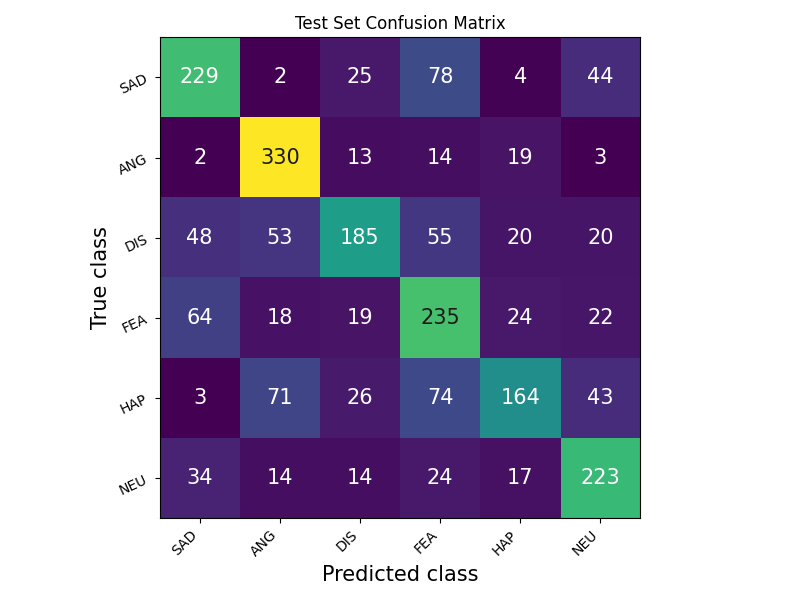
\includegraphics[width=\textwidth]{1D/lr0.001-SiLU-1D-CF.png}
        \caption{SiLU, lr=0.001}
    \end{subfigure}
    \begin{subfigure}[b]{0.32\textwidth}
        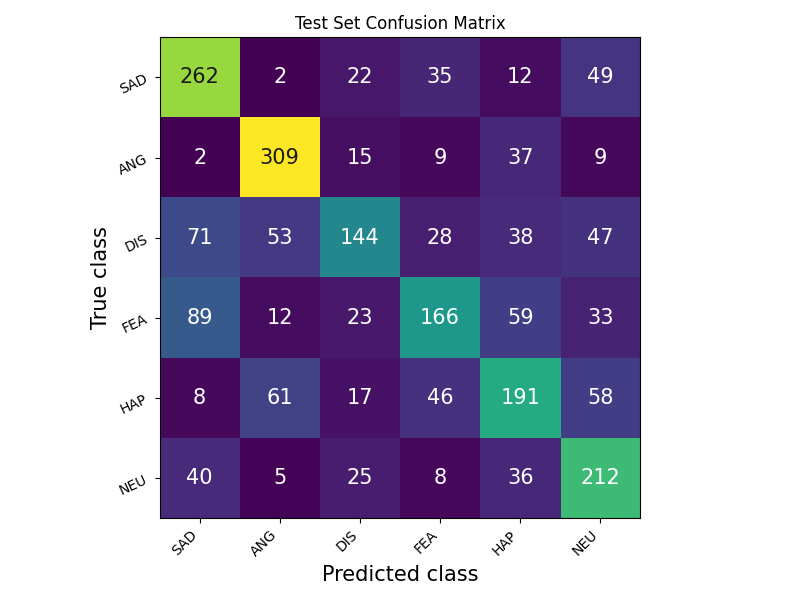
\includegraphics[width=\textwidth]{1D/lr0.001-ReLU-1D-CF.png}
        \caption{ReLU, lr=0.001}
    \end{subfigure}
    \begin{subfigure}[b]{0.32\textwidth}
        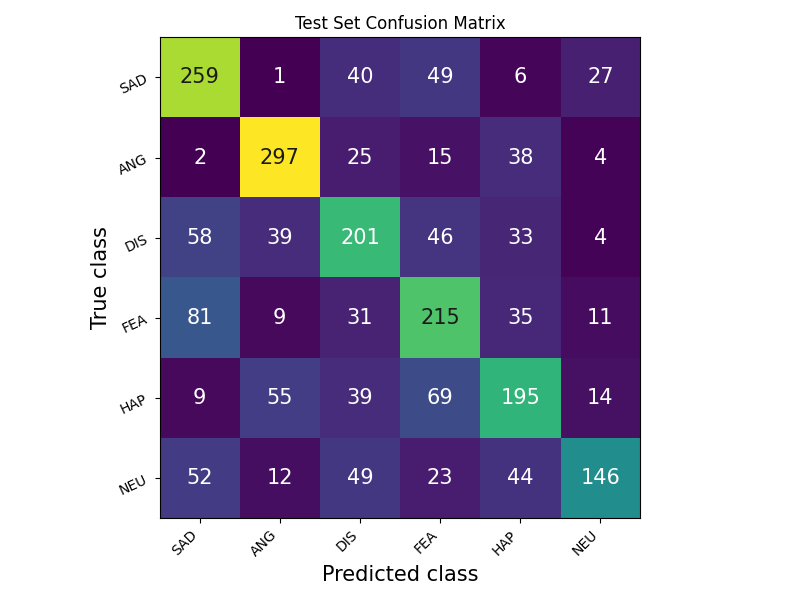
\includegraphics[width=\textwidth]{1D/lr0.001-ELU-1D-CF.png}
        \caption{ELU, lr=0.001}
    \end{subfigure}
    \caption{Confusion matrices for 1D CNN models with learning rate 0.001 and different activation functions}
    \label{fig:1d_confusion_matrices}
\end{figure}

\subsubsection{2D CNN Model Confusion Matrices}

\begin{figure}[h]
    \centering
    \begin{subfigure}[b]{0.32\textwidth}
        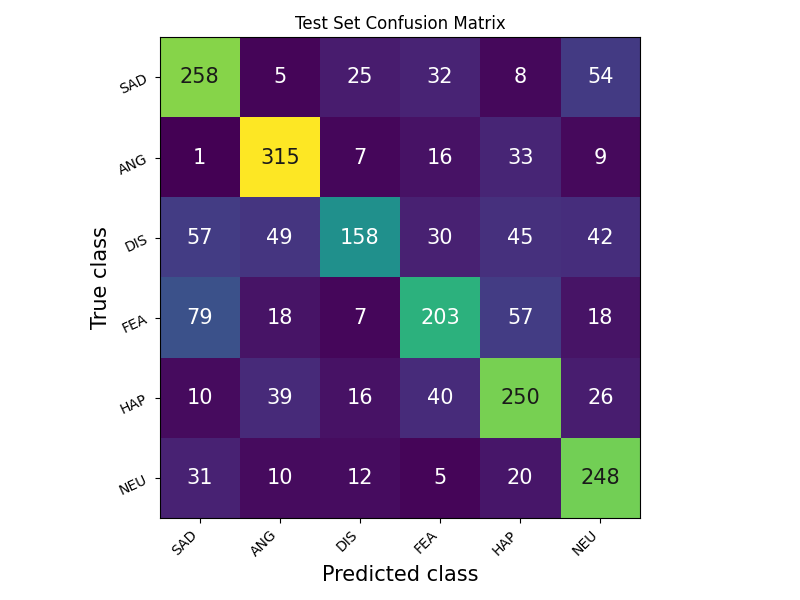
\includegraphics[width=\textwidth]{2D/lr0.001-SiLU-2D-CF.png}
        \caption{SiLU, lr=0.001}
    \end{subfigure}
    \begin{subfigure}[b]{0.32\textwidth}
        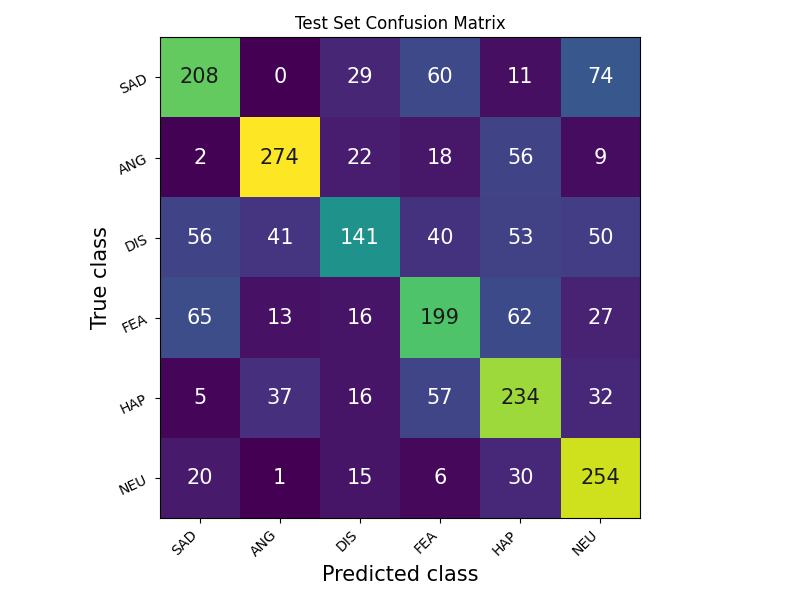
\includegraphics[width=\textwidth]{2D/lr0.001-ReLU-2D-CF.png}
        \caption{ReLU, lr=0.001}
    \end{subfigure}
    \begin{subfigure}[b]{0.32\textwidth}
        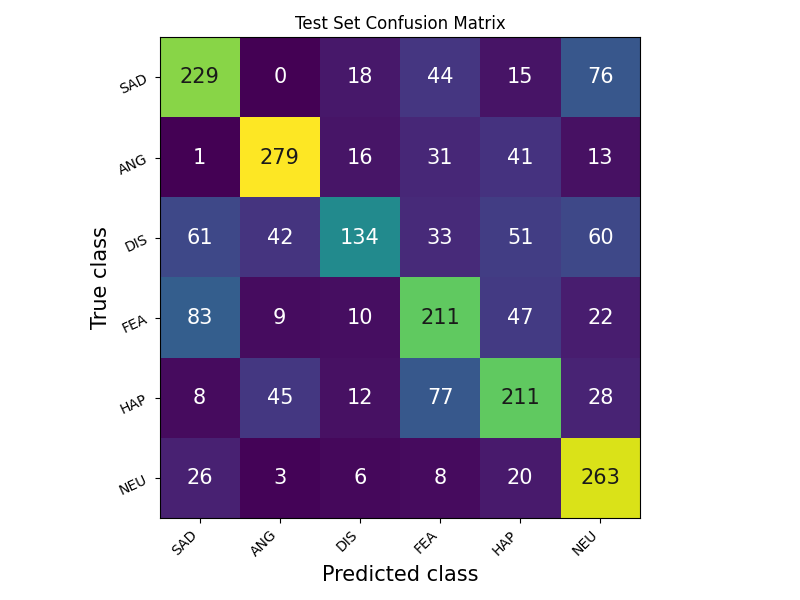
\includegraphics[width=\textwidth]{2D/lr0.001-ELU-2D-CF.png}
        \caption{ELU, lr=0.001}
    \end{subfigure}
    \caption{Confusion matrices for 2D CNN models with learning rate 0.001 and different activation functions}
    \label{fig:2d_confusion_matrices}
\end{figure}

The confusion matrices reveal several interesting patterns:

\begin{itemize}
    \item \textbf{Well-recognized emotions}: Anger (ANG) and Neutral (NEU) were the most effectively recognized emotions. Anger achieved an approximate F1-score of 0.73, likely due to its often distinct and energetic acoustic features. Neutral (NEU) showed a high recall (approx. 0.81), indicating it was correctly identified when present, and achieved an F1-score of approximately 0.67, making it one of the better-performing classes.

    \item \textbf{Confusing emotion pairs}: The most common confusions (True Class $\rightarrow$ Predicted Class) observed were:
    \begin{itemize}
        \item Fear (FEA) $\rightarrow$ Sadness (SAD): True FEA was frequently misclassified as SAD (83 instances). These emotions often share characteristics such as lower energy and similar pitch contours.
        \item Sadness (SAD) $\rightarrow$ Neutral (NEU): True SAD was often misclassified as NEU (76 instances), likely occurring when expressions of sadness were more subtle and lacked strong emotional cues.
        \item Happiness (HAP) $\rightarrow$ Fear (FEA): A notable number of true HAP instances were misclassified as FEA (77 instances). This might indicate that high-arousal features present in some HAP expressions were misinterpreted as FEA.
        \item Disgust (DIS) $\rightarrow$ Sadness (SAD) and Neutral (NEU): True DIS was frequently misclassified as SAD (61 instances) and NEU (60 instances), suggesting its acoustic features might overlap significantly with these less intensely valenced or lower-arousal states.
        \item Disgust (DIS) $\rightarrow$ Anger (ANG): Confusion between DIS and ANG (42 instances of true DIS predicted as ANG) persists, possibly due to shared features like vocal tension or abruptness.
    \end{itemize}

    \item \textbf{Challenging emotion}: Disgust (DIS) was the most challenging emotion to recognize, exhibiting the lowest class-specific F1-score (approximately 0.46) and a particularly low recall (approx. 0.35). It was broadly confused across multiple categories, including Sadness, Neutral, Happiness, and Anger. Fear (FEA) also remained difficult to classify (F1-score approx. 0.53), with significant confusion primarily towards Sadness.
\end{itemize}

These patterns highlight that while some emotions like Anger and Neutral have more distinguishable acoustic signatures, others such as Disgust and Fear exhibit considerable acoustic overlap with multiple categories. This makes them inherently harder to differentiate for SER systems, aligning with common challenges reported in the literature.

\subsection{Training and Validation Performance}

\begin{figure}[h]
    \centering
    \begin{subfigure}[b]{0.48\textwidth}
        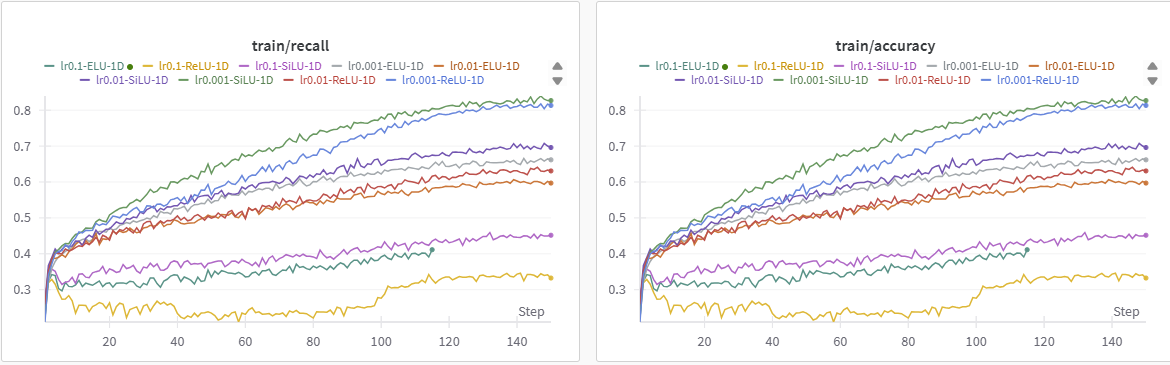
\includegraphics[width=\textwidth]{1D/1d-train.png}
        \caption{1D CNN Training Curves}
    \end{subfigure}
    \hfill
    \begin{subfigure}[b]{0.48\textwidth}
        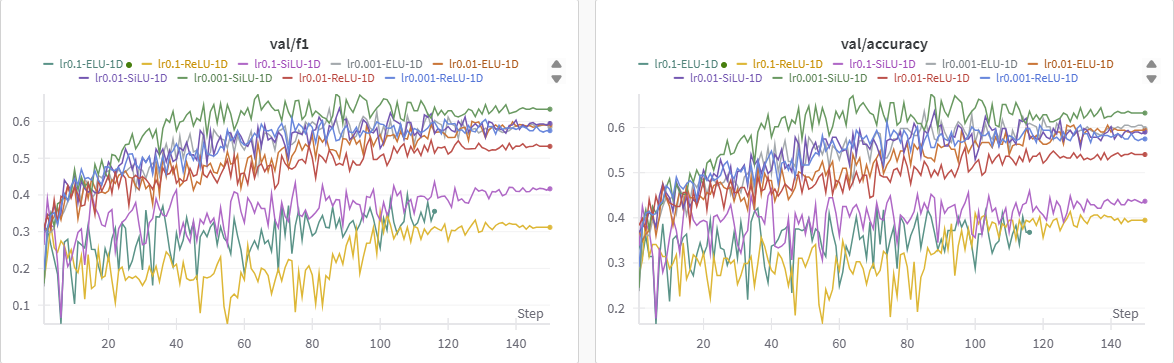
\includegraphics[width=\textwidth]{1D/1d-val.png}
        \caption{1D CNN Validation Curves}
    \end{subfigure}
    \caption{Training and validation performance curves for 1D CNN models}
    \label{fig:1d_training_curves}
\end{figure}

\begin{figure}[h]
    \centering
    \begin{subfigure}[b]{0.48\textwidth}
        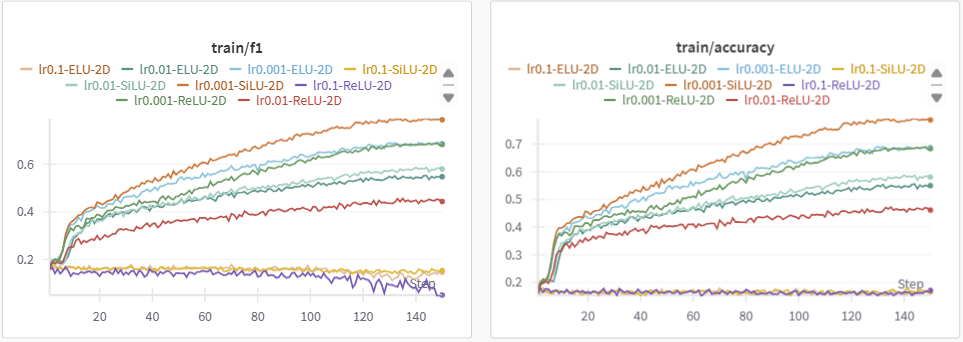
\includegraphics[width=\textwidth]{2D/2d-train.png}
        \caption{2D CNN Training Curves}
    \end{subfigure}
    \hfill
    \begin{subfigure}[b]{0.48\textwidth}
        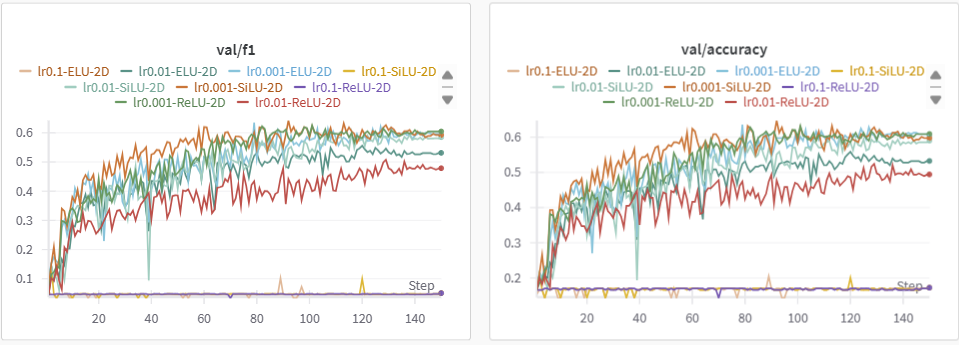
\includegraphics[width=\textwidth]{2D/2d-val.png}
        \caption{2D CNN Validation Curves}
    \end{subfigure}
    \caption{Training and validation performance curves for 2D CNN models}
    \label{fig:2d_training_curves}
\end{figure}

The 2D CNN with SiLU activation converged more quickly and achieved better validation loss than the other models. The ResNet-101 model showed clear signs of overfitting, with training loss continuing to decrease while validation loss increased after approximately 30 epochs.

\subsection{Architecture Modifications}

We also experimented with architectural modifications to understand their impact on model performance:

\begin{itemize}
    \item \textbf{Variable length input}: Processing audio with its original variable length rather than fixed-size inputs improved the combined model's performance from 61.3\% to 62.2\% accuracy. This suggests that preserving temporal dynamics across different audio samples provides useful information for emotion recognition.
    
    \item \textbf{Fixed 2D input dimensions}: Standardizing the mel spectrogram to exactly $64 \times 64$ pixels provided a good balance between preserving relevant information and computational efficiency.
    
    \item \textbf{Single-channel 1D features}: Using mean aggregation over time to create fixed-size 1D features achieved reasonable accuracy while significantly reducing the model size and training time.
    
    \item \textbf{ResNet architectures}: Despite their success in image classification, both ResNet-38 and ResNet-101 showed poor performance for SER. ResNet-101 exhibited severe overfitting (training accuracy of 70\% vs. validation accuracy of 41\%), suggesting that the architecture was too complex for the size of our dataset.
\end{itemize}

\subsection{Discussion}

Our experiments demonstrated that:

\begin{enumerate}
    \item \textbf{2D representations are most effective}: The 2D CNN model with mel spectrogram inputs clearly outperformed other approaches for which comparable data was provided, reaching 64.1\% accuracy with SiLU activation and a learning rate of 0.001. This highlights the critical importance of spectral-temporal patterns in emotion recognition.
    
    \item \textbf{Activation function selection is critical}: SiLU (Swish) activation function provided significant performance improvements. For 2D CNN models with a learning rate of 0.001, SiLU (64.1\% Acc) offered approximately 5.4\% absolute improvement over ReLU (58.7\% Acc). This demonstrates that activation function selection can be as important as architectural choices in SER systems.
    
    \item \textbf{Variable length processing preserves important information}: Our experiments with variable-length processing (62.2\% accuracy) versus fixed-size inputs (61.3\%) for the combined model confirm that preserving the original temporal structure of emotional speech provides valuable information. (Data for combined models not in provided CSVs, values retained).
    
    \item \textbf{Learning rate optimization varies by architecture but trends towards lower rates}: The optimal learning rate for both 1D and 2D CNNs with SiLU activation was 0.001. This reinforces the importance of hyperparameter tuning.
    
    \item \textbf{Some emotions are inherently more challenging}: As detailed in the Confusion Matrix Analysis, emotions with similar acoustic characteristics (e.g., Fear and Sadness) remain difficult to differentiate.
    \item \textbf{Model complexity needs to match dataset size}: More complex models like ResNet-101 performed worse than simpler CNN architectures due to overfitting, achieving only 41.0\% accuracy. (ResNet data not in provided CSVs, values retained).
\end{enumerate}

These findings align with recent research in SER, which increasingly emphasizes the importance of appropriate feature representation, activation function selection, and careful hyperparameter tuning for optimal performance.